% 一维势能束缚态数值解(试射法)
% 定态薛定谔方程|束缚态|数值解|试射法|误差

% 未完成: 把 “数值解一维薛定谔方程(试射法)\upref{NSES} ” 合并过来

\footnote{本词条使用原子单位}我们介绍用试射法解定态薛定谔方程(TISE, Time Independent Schrodinger Equation),其中 $V(x)$ 已知
\begin{equation}
-\frac{1}{2m}\psi(x) + V(x)\psi(x) = E \psi(x)
\end{equation}
要使用 ODE 解算器(如 Matlab 的 ode45), 需要先将上式化为一阶微分方程组
\begin{equation}
\begin{cases}
\psi'(x) = v(x)\\
v'(x) = 2m[V(x) - E]\psi(x)
\end{cases}
\end{equation}

\subsection{对称势能}
先讨论偶函数势能的情况. 当 $V(x)$ 为偶函数时, 定态波函数为奇函数或偶函数. 解 ODE 应该从中点出发, 前者可用初始条件 $\psi(0)=0$, $\psi'(0)=1$, 后者可用初始条件 $\psi(0)=1$, $\psi'(0)=0$. 这样解出来的波函数一般不满足归一化条件, 需要在最后归一化.

现在可用定步长的欧拉法或者龙格库塔四阶法来解 $x\in [0, x_{max}]$ 的薛定谔方程. 显然程序中不能选取 $x\in [0,+\infty]$,但是要保证 $x_{max}$ 足够大,使解出薛定谔方程后有 $\psi(x_{max})\approx 0$, $\psi'(x_{max})\approx 0$.

\subsection{初始条件}
如果势能不是对称的, 我们一般从其中一端作为起始点解微分方程. 若某个小区间 $V(x)$ 看做常数, 解为
\begin{equation}
\psi(x) =
\begin{cases}
\sin(kx) &(E > V)\\
\exp(\kappa x) & (E < V)
\end{cases}
\end{equation}
其中
\begin{equation}
k = \sqrt{2m(E - V)} \qquad
\kappa = \sqrt{2m(V - E)}
\end{equation}
所以 ODE  初始条件选择
\begin{equation}
(\psi(x_0), \psi'(x_0)) =
\begin{cases}
(0, 1) &(E > V(x_0))\\
(\epsilon, \kappa\epsilon) & (E < V(x_0))
\end{cases}
\end{equation}
其中 $\epsilon$ 是一个很小的数. 第二种情况中, 解析初始条件应该是 $(0, 0)$, 但数值解中显然不能用这个. 注意最后归一化以后要检验是否两端都满足 $\psi(x_0) \ll 1$.

\subsection{甩尾法}
如何求得本征值 $E$ 呢?一种简单的方法是试射法. 顾名思义, 取不同离散的 $E$,用一定的条件判断对这些 $E$ 波函数在 $x_{max}$ 处是否满足边界条件 $\psi(x_{max}) \approx 0$\footnote{如果 $x_{max}$ 足够大,只需满足这一条件即可自动满足 $\psi'(x_{max})\approx 0$}.

一般来说,若 $E$ 略大于某本征值 $E_n$ 时,会有 $\psi(x_{max})>0$,略小时会有 $\psi(x_{max})>0$.所以画出 $\psi(x_{max})$ 关于 $E$ 的图像,用目测法找到零点即可. 若需要更精确的本征值, 可选取一个更小的区间,再次画图.

\subsection{中点匹配}
从数值误差来说,从指数末端出射时误差远远大于从指数末端入射. 所以更好的办法是从两端 $x_L, x_R$ 分别入射后在某个中点 $x_M$ 处匹配.

简单的匹配可以采用\textbf{对数导数(log derivative)} 来计算匹配误差, 即
\begin{equation}
\text{err}(E) = \frac{\psi'_L(x_M)}{\psi_L(x_M)} - \frac{\psi'_R(x_M)}{\psi_R(x_M)}
\end{equation}
用多区间二分法即可得到定态能量.

但是这么做有两个缺点, 一是 $\psi(x_M)$ 为零或很小的时候, err 有可能不稳定, 二是用多区间二分法解 $\text{err}(E) = 0$ 有可能出现不收敛的解, 因为该函数存在断点(想象 $\sin(k x_M)$ 的对数导数随 $k$ 变化的情况).

为了解决这个问题, 我们可以构造一个性质更好的函数来代替对数导数, 即用 $\theta$ 表示函数 $\sin x$ 在 $x = \theta$ 处的对数导数
\begin{equation}
\theta = \Arctan(y, y')
\end{equation}
注意对数导数是关于 $\theta$ 的周期函数, 周期为 $\pi$. 只要保证两个 $\theta$ 相同或相差 $n\pi$ 就可以保证对数导数相同.

要构造关于 $\theta$ 的误差函数, 我们可以先计算两个 $\theta$ 之差
\begin{equation}
\theta = \theta_2 - \theta_1 \qquad (\theta \in [-2\pi, 2\pi])
\end{equation}
误差函数 $\opn{err}(\theta)$ 满足一些条件:
\begin{enumerate}
\item $\theta = n\pi$ 为零点(误差函数为零当且仅当对数导数相等)
\item 零点两侧异号(便于用二分法或类似算法求根)
\item 函数连续 (连续性自然是好的)
\item 周期为 $2\pi$ ($\Arctan$ 函数会使 $\theta$ 在 0 到 $2\pi$ 之间突变, 这样可以保证误差函数连续)
\end{enumerate}

一个显然的误差函数是满足这些条件的三角波(也可以用正弦函数, 但是三角波的计算量要小得多).

现在再用多区间二分法\upref{MBisec}就可以解出所有正确的束缚态能量了.

\subsection{检查漏解}
用多区间二分法时, 如果区间划分不够细, 使一个区间中存在多个解, 就会产生漏解. 检查是否漏解可以用波函数节点的数量来判断. 如果波函数的节点数是逐个递增的,则没有漏解. 也就是说第 $n$ 个能级的波函数需要有 $n - 1$ 个节点(不包括两端).

\subsection{Matlab 代码}

完整的代码(\verb|bnd_shoot|)见下文, 作为一个使用的例子, 我们来解一维简谐振子\upref{QSHOxn}.

\begin{lstlisting}[language=matlab, caption=bndShootDemo.m]
close all;
% =====  设置参数  ========
V = @(x) 0.5*x.*x; % 势能
mass = 1; % 质量
xmin = -10; xmid = 0; xmax = 10; % 端点和中点
Espan = [0.1, 10]; % 能量区间
Eresolution = 100; % 二分法区间数
NstepMin = 1000; % ode 解算器最少步数
% =======================

% 画势能曲线
x = linspace(xmin, xmax, 1000);
figure; plot(x, V(x));
xlabel x; title V;

[Eng, X, Psi] = bndShoot(V, xmin, xmid, xmax, mass, Espan, ....
    Eresolution, odeset('RelTol',1e-6, 'MaxStep',abs(xmax-xmin)/NstepMin),...
    true);
\end{lstlisting}

结果如下
\begin{figure}[ht]
\centering
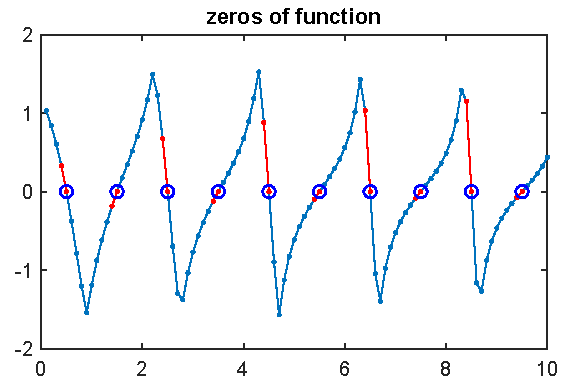
\includegraphics[width=10cm]{./figures/BndSho_1.pdf}
\caption{误差函数零点} \label{BndSho_fig1}
\end{figure}

\begin{figure}[ht]
\centering
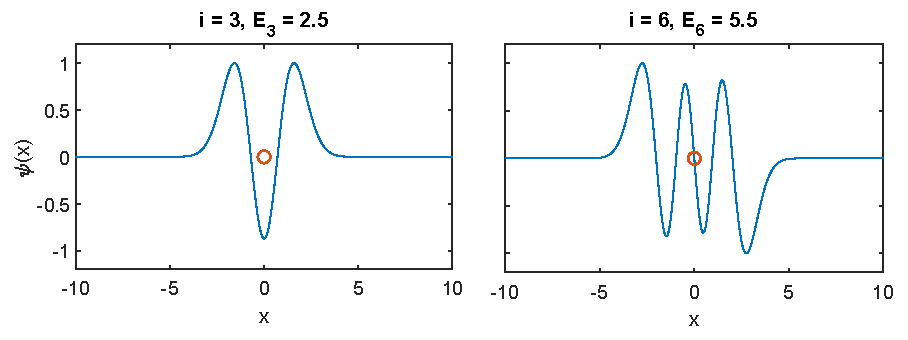
\includegraphics[width=14.5cm]{./figures/BndSho_2.pdf}
\caption{解出的波函数, 这里只给出了第 3 和第 6 个能级, 红点表示左右波函数匹配的位置} \label{BndSho_fig2}
\end{figure}

\begin{lstlisting}[language=matlab, caption=bndShoot.m]
% 求解一维定态薛定谔方程的能级
% 从两端试射
% varargin 是 ode45 解算器的选项
% Eng(i) 是第 i 个能级的能量
% psi(:,i) 是第 i 个能级的波函数
function [Eng, X, Psi] = bndShoot(V, xmin, xmid, xmax, mass, ...
    Espan, EResolution, odeOpt, plot_flag)

% 多区间二分法解出能级和波函数
trial_fun = @(E) bound_shooting_trial(E, V, xmin, xmid, xmax, mass, odeOpt);
Eng = fzeroN(trial_fun, Espan, EResolution);

% 输出, 检查节点个数
X = cell(1,numel(Eng)); Psi = X;
for i = 1:numel(Eng)
    [~, X{i}, Psi{i}] = trial_fun(Eng(i));
    if numzero(Psi{i}) > i - 1
        warning(['missed bound state ', num2str(i),...
            ', increase Eresolution!']);
    elseif numzero(Psi{i}) < i - 1
        error('duplicate bound state found!');
    end
    
    if plot_flag
        x = X{i}; psi = Psi{i};
        figure; plot(x,psi); axis([x(1),x(end),-1.2,1.2]);
        hold on;
        xlabel('x'); ylabel('\psi(x)');
        Nzeros = numzero(psi);
        title(['i = ', num2str(i),...
            ', E_{', num2str(Nzeros+1), '} = ',  num2str(Eng(i))]);
        scatter(xmid,0);
    end
end
end

% 单个能量试射
% 输出误差函数和其他信息
function [err, x, psi, th1, th2] = bound_shooting_trial(E, V, ...
    xmin, xmid, xmax, mass, odeOpt)
dy = 1e-16; % dy = psi(xmin) 和 psi(xmax)
[x1, Y1] = bound_shooting_left(E, V, [xmin,xmid], mass, dy, odeOpt);
[x2, Y2] = bound_shooting_right(E, V, [xmax,xmid], mass, dy, odeOpt);

% 误差
[err, th1, th2] = fmatch_err(Y1(end,1),Y1(end,2),Y2(end,1),Y2(end,2));

psi1_max = max(abs(Y1(:,1)));
psi2_max = max(abs(Y2(:,1)));

% 波函数 (max(psi) = 1)
if nargout > 1
    x = [x1; flip(x2(1:end-1))].';
end
if nargout > 2
    v1 = Y1(end,:);
    v2 = Y2(end,:);
    scale = sign(dot(v1,v2))*norm(v1)/norm(v2);
    if psi1_max >= psi2_max * abs(scale)
        psi = [
            Y1(:,1).' / psi1_max,  .....
            flip(Y2(1:end-1,1)).' * (scale / psi1_max)];
    else
        psi = [
            Y1(:,1).' / (scale * psi2_max),  .....
            flip(Y2(1:end-1,1)).' / psi2_max];
    end
end
end

% 从左边入射(使用 ode45 解算器)
function [x, Y] = bound_shooting_left(E, V, xspan, mass, dy, odeOpt)
if V(xspan(1)) > E
    Y0 = [1; sqrt(2*mass*(V(xspan(1)) - E))] * dy;
else
    warning('起始点 E > V, 确定吗?');
    Y0 = [0; 1];
end
odefun = @(x,Y) TISE_odefun(x,Y,E,V,mass);
[x,Y] = ode45(odefun, xspan, Y0, odeOpt);
end

% 从右边入射
function [x, Y] = bound_shooting_right(E, V, xspan, mass, dy, odeOpt)
if V(xspan(1)) > E
    Y0 = [1; -sqrt(2*mass*(V(xspan(1)) - E))] * dy;
else
    warning('起始点 E > V, 确定吗?');
    Y0 = [0; 1];
end
odefun = @(x,Y) TISE_odefun(x,Y,E,V,mass);
[x,Y] = ode45(odefun, xspan, Y0, odeOpt);
end

% ode 函数
% 由 Y = [psi(x); psi'(x)] 求 dY(x) = [psi'(x), psi''(x)]
function dY =TISE_odefun(x,Y,E,V,mass)
dY(2,1) = 2*mass*(V(x)-E)*Y(1);
dY(1) = Y(2);
end

% 多区间二分法求函数零点
function roots = fzeroN(fun,interval,resolution,converge,options)
if ~exist('converge','var') || isempty(converge)
    converge = false;
end
if ~exist('options','var')
    options = optimset;
end
x=linspace(interval(1),interval(end), resolution);
y=arrayfun(fun,x);
figure; plot(x,y,'.-'); hold on;
title('the function to be found zeros of');
[Nind, ind] = numzero(y);

roots=zeros(1, Nind); kk = 0;
for ii=1:Nind
    plot([x(ind(ii)),x(ind(ii)+1)], ...
        [fun(x(ind(ii))),fun(x(ind(ii)+1))], '.-r');
    root = fzero(fun,[x(ind(ii)),x(ind(ii)+1)], options);
    if ~converge || converge && iszero(fun,root,options.TolX)
        kk = kk + 1;
        roots(kk) = root;
        scatter(root, fun(root), 'b');
    end
end
roots = roots(1:kk);
end

% 计算两函数在某点匹配的误差
function [err, th1, th2] = fmatch_err(y1,dy1,y2,dy2)
th1 = atan2(y1,dy1);
th2 = atan2(y2,dy2);
err = mod(th2 - th1, 2*pi);
if err > 0.5*pi && err <= 1.5*pi
    err = pi - err;
elseif err > 1.5*pi
    err = -2*pi + err;
end
end

% 数函数的零点
function [N, ind] = numzero(y)
Sign=sign(y);
ind=find(Sign(1:end-1).*Sign(2:end)<0);
N = numel(ind);
end
\end{lstlisting}
